\documentclass [11pt]{article}
\usepackage[left=1in, right=1in, top=1in, bottom=1in]{geometry}

\usepackage{titling}
\usepackage{lipsum}
\usepackage[utf8]{inputenc}
\usepackage{geometry}
\usepackage{float}
\usepackage{titlesec}
\usepackage{titling}
\usepackage{graphicx}
\usepackage{amsmath}
\usepackage{amssymb}
\usepackage{DejaVuSansMono}
\usepackage[parfill]{parskip}
\usepackage[autostyle=false, style=english]{csquotes}
\MakeOuterQuote{"}
\geometry{total={240mm,320mm},
          left=25mm,right=25mm,%
          bindingoffset=0mm, top=25mm,bottom=25mm}


\floatstyle{boxed} 
\restylefloat{figure} % Makes floats have a frame

% \renewcommand{\ttdefault}{DejaVuSansMono-TLF}
% \renewcommand{\rmdefault}{lmss}
\linespread{1}
\newcommand{\linia}{\rule{\linewidth}{0.2pt}}

\titlespacing\section{0pt}{12pt plus 4pt minus 2pt}{0pt plus 2pt minus 2pt}

\makeatletter
\def\@maketitle{%
\nopagebreak[4]
  \vspace*{-\topskip}      % remove the initial space
  \begingroup\centering    % instead of \begin{center}
  \let \footnote \thanks
  \hrule height \z@        % to avoid the insertion of lineskip glue
    {\huge \@title \par}%
    \vskip 0.5em 
    {\large
      \lineskip .5em 
      \begin{tabular}[t]{c}%
        \@author 
      \end{tabular}\par}%
    % \vskip 1em 
    % {\large \@date}%
  \par\endgroup            % instead of \end{center}
  \let\endtitlepage\relax\let\endtitlepage\relax
  \vskip 1.5em             % <--- modify this to adjust the separation
\large}
\makeatother


\begin{document}
\inputencoding{utf8}
\title{ Heuristic Opt. Techniques - Assignment 1 Report}
\author{ Martin Blöschl and Cem Okulmus }

\maketitle
\thispagestyle{empty}

\section{Summary}
We chose a simple two-step algorithm that constructs an initial solution. First, the ordering is fixed by looking at the order of the vertices. We found out that the algorithm gives the best results when we place the vertices with the highest degree at the top and bottom of the spine. Then, the edges are one by one added to the page with the minimal new crossings.
 As for the randomization, we found ways to extends these steps to allow for a parameterized uncertainty factor (similar to the $\alpha$ factor in GRASP). 
Our results showed that randomization improved our results for almost all our test instances. 

\section{Implementation}

In the following subchapters we will describe details of the implementation.

\subsection{Solution representation}
Internally, we represent a solution as the order of its vertices, an integer array, and the lists of edges assigned to pages. 

Additionally, we developed a new data structure that stores the active edges at each vertex. For example, a edge (0,7) would be active at all vertices between the vertex 0 and vertex 7. Even though this increases space consumption, we are able to answer crossing-queries in very little time. If we want to add a new edge we only look at the active edges at the beginning and the end of the new edge and can get the number of newly introduced crossings in logarithmic time.

\subsection{Two step algorithm}

We decided that our construction heuristic should first fix the vertex order and afterwards determine a good page partition for this ordering. This allowed us to find clear rules for the construction at each step, as we will explain in the following sections. A downside of this method is that it does not allow to avoid certain crossings encountered during the heuristic by changing the vertex order. This could be alleviated by adding a local search procedure, ideally searching for both changes in vertex ordering and page partition. 

Furthermore, fixing the vertices first allows us to create the active edge data structure (see above), and thus lets us very efficiently check whether adding an edge would introduce new crossings. We think that this operation is used very often (and also used in further extensions like local search) and therefore this approach seems to be the most promising.


\subsection{Deterministic Construction}

Our deterministic construction looks at the degree of each vertex to determine its order. The idea here is to have vertices with higher degree nearer the middle of the ``spine'', as shown in the graph below. 
\begin{center}
    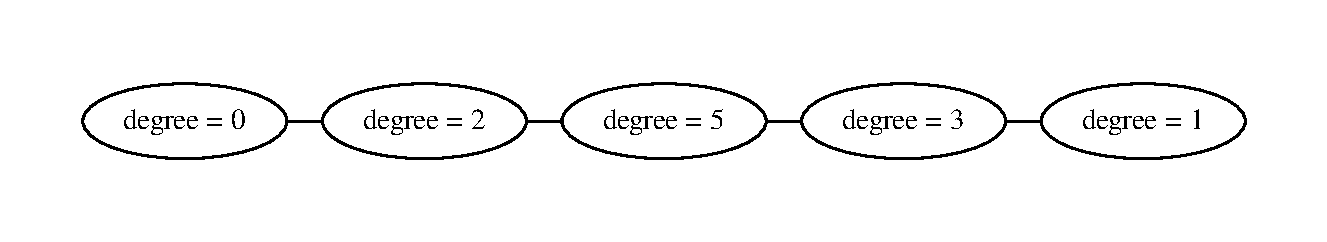
\includegraphics[scale=0.6]{bilder/graph.pdf}
\end{center}
The idea here is that since most edges will be incident to the degrees in the middle, there will be less crossings. 

For the edge partitioning, we implemented a first fit algorithm that chooses the first page with which the new edge introduces no new crossings. If no such page exists, the one with the least introduced crossings is chosen. 

\subsection{Randomized construction}
For the randomization, we tried to find meaningful ways to introduced a controlled randomization factor into each step, that does not automatically regress to a random search. For this purpose, we used a parameter $\alpha$. $\alpha = 0.0$  means the algorithm proceeds as the deterministic case, with $\alpha = 1.0$ essentially reducing each to step to be almost completely random. Every value in between gradually changes the behavior. 

For the vertex ordering, a random offset for the degree count is added. The vertices are then sorted by degree and offset together. 

As for the edges, we first collect all edges to be added and then shuffle the order in which the first fit procedure from above is considered. We experimented with also adding edges randomly (depending on $\alpha$), but the results proved not satisfiable. 

\section{Evaluation}
Our tests were run mostly on our private machines. This is a laptop with an Intel i7-4500U @ 1.8 GHz and 8 GB of RAM running Ubuntu  16.04 x64  and a desktop PC with an Intel Core 2 Quad Q6600 and 6GB of RAM on Windows 10 x64. We used the Java Framework as a starting point and implemented it in Java 8. 

Our best results can be seen on the tool provided to submit solutions. We found that the best results were almost always achieved by the randomized variant (except for instance 10, where our best result stems from the deterministic version). When sampling for 10 values, however, it can be seen that the randomized construction usually is worse on average. The minimum is almost always lower, however.

\begin{figure}[H]
\centering
  \begin{tabular}{| c | c | c | c |}
\hline
Instance name & Deterministic Construction & Randomized Mean & Randomized Std. Deviation \\
\hline
Instance 1 & 18 & 18.5 & 3.75 \\
\hline 
Instance 2 & 59 & 68.6 & 10.67 \\
\hline 
Instance 3 & 114 & 132.9 & 26.49 \\
\hline 
Instance 4 & 215 & 160.02 & 26.31 \\
\hline 
Instance 5 & 91 & 89.2  & 23.4 \\
\hline 
Instance 6 & 6732459 & 4498075 & 211133\\
\hline 
Instance 7 & 156906 & 157854 & 5740.4 \\
\hline 
Instance 8 & 915429 & 633363 & 19867 \\
\hline 
Instance 9 & 1529691 & 789895 & 71314 \\
\hline 
Instance 10 & 107333 & 121714 & 3317.5 \\
\hline 
\end{tabular}
\caption{Test results of crossing counts.  10 samples were used for randomized part}
\end{figure}




We assume the most obvious way to improve our results would be the implementation of a local search. Since we implemented an incremental way to detect crossings (the most computationally expensive part of our heuristic), we could quickly introduce changes to the page partition (though not the vertex order) and check for improvements. 



\end{document}